\documentclass[working, oneside]{../../Preambles/tuftebook}
% Import xcolor and define some colors
\usepackage{{xcolor}}
\definecolor{{background}}{{HTML}}{{{background}}}
\definecolor{{foreground}}{{HTML}}{{{foreground}}}
\definecolor{{math}}{{HTML}}{{{color6}}}

%%%%%%%%%%%%%%%%%%%%%%%%%%%%%%%%%%%%%%%% IMPORTS %%%%%%%%%%%%%%%%%%%%%%%%%%%%%%%%%%%%%%%%
\documentclass[11pt,onesize,a4paper,titlepage]{article}

%%%%%%%%%%%%%%% Formatting %%%%%%%%%%%%%%% 
\usepackage[english]{babel}
\usepackage[utf8]{inputenc}
\usepackage{adjustbox}
\usepackage{geometry} % Margins
\usepackage{sectsty} % Custom Sections

%%%%%%%%%%%%%%% Font %%%%%%%%%%%%%%% 
\usepackage{Archivo}
\usepackage[T1]{fontenc}
\sffamily

%%%%%%%%%%%%%%% Graphics %%%%%%%%%%%%%%% 
\usepackage{fontawesome5} % Icons
\usepackage{graphicx} % Images
\usepackage[most]{tcolorbox} % Color Box
\usepackage{xcolor} % Colors
\usepackage{tikz} % For Drawing Shapes
%%%\usepackage{emoji} % For flags
\tcbuselibrary{breakable}
%%%\usepackage{academicons}

%%%%%%%%%%%%%%% Miscelanous %%%%%%%%%%%%%%% 
\usepackage{lipsum} % Lorem Ipsum
\usepackage{hyperref} % For Hyperlinks

%%%%%%%%%%%%%%% Colors %%%%%%%%%%%%%%% 
\definecolor{title}{HTML}{b5bff5} % Color of the title
\definecolor{bars}{HTML}{889af0} % Color of the title
\definecolor{backdrop}{HTML}{f2f2f2} % Color of the side column
\definecolor{lightgray}{HTML}{dfdfdf} % Color for the skill bars

%%% TU green: #639a00
%%% TU gray: #e6e6e6
%\definecolor{title}{HTML}{639a00} % Color of the title TU
%\definecolor{bars}{HTML}{889af0} % Color of the title TU

% \definecolor{backdrop}{HTML}{f2f2f2} % Color of the side column
\definecolor{backdrop}{HTML}{e6e6e6} % Color of the side column

\definecolor{subtitle}{HTML}{606060} % 


%%%%%%%%%%%%%%% Section Format %%%%%%%%%%%%%%% 
\sectionfont{                     
    \LARGE % Font size
    \sectionrule{0pt}{0pt}{-8pt}{1pt} % Rule under Section name
}

\subsectionfont{
    \Large % Font size
    \fontfamily{phv}\selectfont % Font family
    %\sectionrule{0pt}{0pt}{-8pt}{1pt} % Rule under Subsection name
    \sectionrule{5pt}{0pt}{0pt}{0pt} % Rule under Subsection name
}

%%%%%%%%%%%%%%% Margins and Headers %%%%%%%%%%%%%%%
\geometry{
  a4paper,
  left=7mm,
  right=7mm,
  bottom=10mm,
  top=10mm
}

\pagestyle{empty} % Empty Headers

\usepackage{marvosym}

% \renewcommand\qedsymbol{\CoffeeCup}

\usepackage{changepage}

\newenvironment{subexercise}[1]{%
    \begin{mdframed}[linewidth=0.5pt, linecolor=foreground, backgroundcolor=background, leftmargin=0cm, innerleftmargin=1em, innertopmargin=0pt, innerbottommargin=0pt, innerrightmargin=0pt, topline=false, rightline=false, bottomline=false]
    \par\noindent\textcolor{foreground}{\textbf{#1.}}\hspace{1em}\ignorespaces
}{%
    \par\addvspace{\baselineskip}\end{mdframed}\ignorespacesafterend
}
\newenvironment{solution}{%
    % \par\addvspace{\baselineskip}\noindent\makebox[\textwidth]{\textcolor{foreground}{\textbullet\hspace{1em}\textbullet\hspace{1em}\textbullet}}\par\addvspace{\baselineskip}
    \begin{mdframed}[linewidth=0.5pt, linecolor=foreground, backgroundcolor=background, rightmargin=0cm, innerleftmargin=0cm, innertopmargin=0pt, innerbottommargin=0pt, innerrightmargin=1em, topline=false, leftline=false, bottomline=false]
    \par\noindent\textcolor{foreground}{\textit{Solution.}}\hspace{1em}\ignorespaces
}{%
    \par\addvspace{\baselineskip}\noindent\hfill\textcolor{foreground}{\Coffeecup}\par\addvspace{\baselineskip}\end{mdframed}\ignorespacesafterend
}
% Exercise environment

\declaretheoremstyle[
    name= \textcolor{foreground}{Exercise},
    postheadspace = \newline,
    bodyfont = \normalfont\color{foreground},
    postheadhook={\textcolor{math}{\rule[.4ex]{\linewidth}{0.5pt}}\\},
    % numberwithin=chapter,
    mdframed={
        backgroundcolor = background,
        linecolor = foreground,
        linewidth = 0.5pt,
        rightline =  true,
        topline = true,
        bottomline = true,
        skipabove=20pt,
        skipbelow=20pt,
        innerleftmargin=15pt,
        innertopmargin=10pt,
        innerrightmargin=15pt,
        innerbottommargin=10pt}
    ]{exercise}
\declaretheorem[style=exercise,numbered=no]{exercise}

% \etocsetlevel{exercise}{2}

% \AtEndEnvironment{exercise}{%
%   \etoctoccontentsline{exercise}{\protect\numberline{\theexercise}}%
% }%
% \etocsetstyle{exercise}
% {}
% {}
% % this will be rendered like a non-numbered section, but we could have used
% % \numberline here also
% {\etocsavedsectiontocline{Exercise \etocnumber}{\etocpage}}
%     {}

% theorem environment

\declaretheoremstyle[
    name= \textcolor{foreground}{Theorem},
    postheadspace = \newline,
    bodyfont = \normalfont\color{foreground},
    postheadhook={\textcolor{math}{\rule[.4ex]{\linewidth}{1pt}}\\},
    mdframed={
        backgroundcolor = background,
        linecolor = foreground,
        linewidth = 1pt,
        rightline =  true,
        topline = true,
        bottomline = true,
        skipabove=20pt,
        skipbelow=20pt,
        innerleftmargin=15pt,
        innertopmargin=10pt,
        innerrightmargin=15pt,
        innerbottommargin=10pt}
    ]{theorem}
\declaretheorem[style=theorem,numbered=yes]{theorem}

\declaretheoremstyle[
    name= \textcolor{foreground}{Definition},
    postheadspace = \newline,
    bodyfont = \normalfont\color{foreground},
    postheadhook={\textcolor{math}{\rule[.4ex]{\linewidth}{1pt}}\\},
    mdframed={
        backgroundcolor = background,
        linecolor = foreground,
        linewidth = 1pt,
        rightline =  true,
        topline = true,
        bottomline = true,
        skipabove=20pt,
        skipbelow=20pt,
        innerleftmargin=15pt,
        innertopmargin=10pt,
        innerrightmargin=15pt,
        innerbottommargin=10pt}
    ]{definition}
\declaretheorem[style=definition,numbered=yes]{definition}
% Example environment

\declaretheoremstyle[
name= \quad \underline{Proof:},
     headfont = \bfseries\sffamily,
     postheadspace = \newline,
     % notebraces = \bfseries{(}{)a},
     headpunct = {},
     bodyfont = ,
     postheadhook={\textcolor{foreground}{\rule[0.4ex]{\linewidth}{0pt}}\\},
     qed=\qedsymbol,
    % spacebelow = 10pt,
    mdframed={
  backgroundcolor = background,
  linecolor = foreground,
  linewidth = 1pt,
  skipabove=10pt,
  skipbelow=10pt,
  rightline = false,
  topline = false,
  leftline = false,
  bottomline = false,
  innerleftmargin=15pt,
  innertopmargin=15pt,
  innerrightmargin=15pt,
  innerbottommargin=15pt}
]{pro}
    % \declaretheorem[style=pro,numbered=no]{Proof}

\declaretheoremstyle[
name= \quad \underline{\textcolor{foreground}{Example}},
     headfont = \bfseries\sffamily,
     postheadspace = \newline,
     % notebraces = \bfseries{(}{)a},
     headpunct = {},
     bodyfont = \normalfont\color{foreground},
     postheadhook={\textcolor{foreground}{\rule[0.4ex]{\linewidth}{0pt}}\\},
     % spacebelow = 10pt,
    mdframed={
  backgroundcolor = background,
  linecolor = foreground,
  linewidth = 1pt,
  skipabove=10pt,
  skipbelow=10pt,
  rightline = false,
  topline = false,
  leftline = false,
  bottomline = false,
  innerleftmargin=15pt,
  innertopmargin=15pt,
  innerrightmargin=15pt,
  innerbottommargin=15pt}
]{ex}
\declaretheorem[style=ex,numbered=no]{example}

\declaretheoremstyle[
     name=,
     headfont = \bfseries\sffamily,
     notebraces = \bfseries{},
     headpunct = { -},
     bodyfont = \color{foreground}\normalfont,
     % postheadhook={\textcolor{black}{\rule[.4ex]{\linewidth}{0.2pt}}\\},
    % spacebelow = 10pt,
    mdframed={
  backgroundcolor = background,
  linecolor = foreground,
  linewidth = 1pt,
  skipabove=0pt,
  skipbelow=0pt,
  innerleftmargin=10pt,
  innertopmargin=10pt,
  innerrightmargin=10pt,
  innerbottommargin=10pt,
  rightline = false,
  topline = false,
  leftline = false,
  bottomline = true}
]{subexercise}
% \declaretheorem[style=subexercise,numbered=no]{subexercise}

\declaretheoremstyle[
     name= \color{losning}Løsning,
     headfont = \bfseries\sffamily,
     notebraces = \bfseries{},
     postheadspace = \newline,
     headpunct = {:},
     bodyfont = \normalfont,
     % qed = ,
     % postheadhook={\textcolor{black}{\rule[.4ex]{\linewidth}{0.2pt}}\\},
    % spacebelow = 10pt,
    mdframed={
  backgroundcolor = background,
  linecolor = losning!75,
  linewidth = 1pt,
  skipabove=0pt,
  skipbelow=10pt,
  innerleftmargin=10pt,
  innertopmargin=10pt,
  innerrightmargin=10pt,
  innerbottommargin=10pt,
  leftline = false,
  rightline = true,
  topline = false,
  bottomline = true}
]{solution}

\newenvironment{SimpleBox}[1]{%
  \begin{mdframed}%
    \noindent\textbf{#1}\\[1ex]
}{%
  \end{mdframed}%
}


\begin{document}
\let\cleardoublepage\clearpage
\thispagestyle{fancy}
\chapter{Handin 7 - 10 ECTS}
\textit{We have used Generative Artificial Intelligence tools in doing this
assignment, for the following legitimate use cases only: to get background
information or understand the topic / problem, to improve writing of own
text, to find gaps in our knowledge. The solution of the assignment is
entirely our own.}
\begin{exercise}[a]
You are given a collection of three short documents:
\begin{enumerate}
    \item \textit{The sky is blue.}
    \item \textit{The sun is bright.}
    \item \textit{The sun in the sky is bright.}
\end{enumerate}
Please calculate the TF-IDF score for the word “sky” for each of the documents. Make sure to include the intermediate steps of your calculation in your solution.
\end{exercise}
The TF-IDF score is a combinantion of the term-frequency and the inverse document frequency. It is calculated in the following way,
\begin{SimpleBox}{TF-IDF}
    Given a term $i$ and document $j$, the term frequency $TF_{ij}$ is given by,
    \[
    TF_{ij} = \frac{f_{ij}}{\sum_i f_{ij}}
    .\] 
    Where $f_{ij}$ is the frequency of the term $i$ in the document $j$, which is normalized by the sum of all the frequencies of any other terms. The inverse document frequency is given by,
    \[
    IDF_{i} = \log \frac{N+1}{n_i +1}
    .\] 
    Where $N$ is the total number of documents, and $n_i$ is the number of documents that mention the term $i$. The TD-IDF score is found by multiplying the two,
     \[
    w_{ij} = TF_{ij} \cdot IDF_{i}
    .\] 
\end{SimpleBox}
We start by calculating the $IDF$ score for the term  \textit{sky}, as this only has to be calculated once for all the documents,
\[
IDF_{sky} = \log \frac{N+1}{n_{sky}+1} = \log \frac{3}{2}
.\] 
To calculate the TF-scores, we essentially have to count the number of terms in each of the documents and use that as our normalization factor. But before doing so, we should filter out non-significant. I have chosen the following words as insignificant,
\[
\text{insignificant\_words} = \left\{ \text{is, The, in, the} \right\} 
.\] 
The $TF_{sky, j}$ scores for the three are,
\begin{align*}
    TF_{sky, 1} = \frac{1}{2} \quad, \quad
    TF_{sky, 2} = \frac{0}{2} = 0 \quad,\quad
    TF_{sky, 3} = \frac{1}{3}
.\end{align*}
Combining $TF$ and $IDF$ we get,
 \begin{align*}
    w_{sky, 1} = \frac{1}{2}\log \frac{3}{2} \quad, \quad    w_{sky, 2} =0 \quad, \quad    w_{sky, 3} =\frac{1}{3}\log \frac{3}{2} \quad, \quad
.\end{align*}
So document 1 is the most relevant, document 2 is completely irrelevant and document 3 is somewhat relevant.
\begin{exercise}[b]
Assume we have 2 documents:
\begin{enumerate}
    \item The vector for the first document is $(1,1,1,1,1,1,0,0)$
    \item The vector for the second document is $(0,1,0,1,1,1,1,1)$
Please calculate the document similarity using cosine similarity. Make sure to include the intermediate steps of your calculation in your solution.
\end{enumerate}
\end{exercise}
The cosine similarity is calculated in the following way,
\begin{SimpleBox}{Cosine similarity}
    The \textit{cosine similarity} $Q_{ab}$ of two vectors $a$ and $b$ is given by,
     \[
    Q_{ab} = \frac{a \cdot b}{\|a\|\|b\|}
    .\] 
\end{SimpleBox}
Lets start by calculating the dot product where $a = (1,1,1,1,1,1,0,0)^{T}$ and $b =(0,1,0,1,1,1,1,1)^{T}$
\[
a\cdot b = 4
.\] 
And the norm of each,
\[
\|a\| = \|b\|=\sqrt{6} 
.\] 
So $Q_{ab}$ is found to be,
\[
Q_{ab} = \frac{4}{\sqrt{6} ^2} = \frac{2}{3}
.\]  
\newpage
\begin{exercise}[c]
 Consider the following graph representation of six web pages 1,…,6 and the
hyperlinks between them. Initially, all these web pages have the same PageRank
score which is 1/6. Please calculate the PageRank of all the nodes for the next
iteration. Make sure to include the intermediate steps of your calculation in your
solution
\end{exercise}
\begin{figure}[htpb]
    \centering
    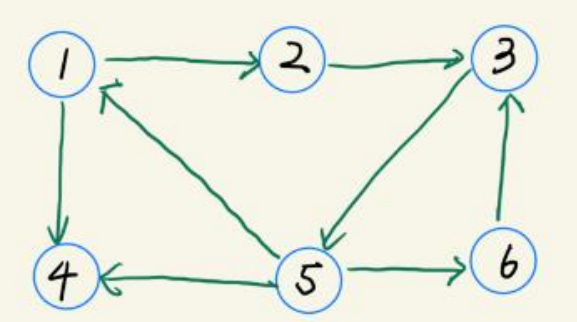
\includegraphics[width=0.5\textwidth]{afl7.png}
\end{figure}
We use the pagerank formula,
\begin{SimpleBox}{PageRank}
    Given a directional graph, the rank $P$ of the node $A$ is given by,
    \[
    P\left( A \right) = \sum_i \frac{P\left( X_i \right) }{O\left( X_i \right) }
    .\] 
    Where $X_i$ are the nodes pointing to $A$, and $O\left( X_i \right) $ is the number of vertices leaving $X_i$
\end{SimpleBox}
During a single iteration, we calculate the scores of all the nodes using the initial state. The page rank of each node is then updated at the end of the iteration (this is at least what was done in the example in the slides). For a bigger graph, it would make sense to update the pageranks at some intermediate steps. Since all our nodes are in the initial state we have,
\[
P\left( X_i \right) = \frac{1}{6} \quad\quad \text{for all }i
.\] 
The pagerank of each node can then be calculated as,
\begin{align*}
    P\left( X_1 \right) &= \frac{P\left( X_5 \right) }{O\left( X_5 \right) } = \frac{1}{6}\cdot \frac{1}{3} = 0.55\\
    P\left( X_2 \right) &= \frac{P\left( X_1 \right) }{O\left( X_1 \right) } = \frac{1}{6}\cdot \frac{1}{2}= 0.083\\
    P\left( X_3 \right) &= \frac{P\left( X_2 \right) }{O\left( X_2 \right) }+ \frac{P\left( X_6 \right) }{O\left( X_6 \right) } = \frac{1}{6} + \frac{1}{6}=0.33\\
    P\left( X_4 \right) &= \frac{P\left( X_4 \right) }{O\left( X_4 \right) } + \frac{P\left( X_5 \right) }{O\left( X_5 \right) } = \frac{1}{6}\cdot \frac{1}{2} + \frac{1}{6}\cdot \frac{1}{3}=0.13\\
    P\left( X_5 \right) &= \frac{P\left( X_3 \right) }{O\left( X_3 \right) } = \frac{1}{6}= 0.166\\
    P\left( X_6 \right) &= \frac{P\left( X_5 \right) }{O\left( X_5 \right) } = \frac{1}{6}\cdot \frac{1}{3}=0.055
.\end{align*}
Which gives us the following ranking from highest to lowest: $\left( X_3, X_5, X_4, X_2, X_1, X_6 \right) $
\begin{exercise}[d]
Consider a scenario where we are asked to develop a diagnostic tool for a
serious disease by finding relevant medical literature. Failing to identify
information about a sick patient could be life-threatening, but providing nonrelevant information would only be a minor irritation.
\end{exercise}
\begin{subexercise}{}
In this case, which is more important: precision or recall? Please argue for
your choice.
\end{subexercise}
In this case, recall is the most important. A high recall with low precision, is likely to return some cases that aren't relevant, but should find most relevant cases. On the other having high precision with low recall, will return a sample dense in relevant cases, but is likely to forget some relevant cases. As missing relevant cases is deadly, the first error is preferable in this case.
\begin{subexercise}{}
Given the following summary of the retrieval results, please calculate the
recall, precision, and F1 score. Make sure to include the intermediate steps
of your calculation in your solution.
\begin{itemize}
    \item 95 relevant medical documents were retrieved.
    \item 30 irrelevant documents were retrieved.
    \item 5 relevant medical documents were missed.
    \item 22 irrelevant documents were not retrieved.
\end{itemize}
\end{subexercise}
The different scores are defined in the following way,
\begin{SimpleBox}{Recall, Precision and F1 scores}
    Let $R$ be the recall score and $P$ the prescision score. Let $D$ be the number of documents,  $D_p$ the relevant documents, $D_f$ the irrelevant documents and  $D_r$ and $D_m$ the retrieved and missed/not retrieved documents. The scores are then found by,
     \begin{align*}
         R& = \frac{D_{rp}}{D_p} \\
        P &= \frac{D_{rp}}{D_r} \\
        F_1 &= \frac{2RP}{P + R}
    .\end{align*}
\end{SimpleBox}
In our case we have, 
\begin{align*}
    D_{rp} &= 95 \\
    D_p &= D_{rp} + D_{mp} = 5 + 95 = 100 \\
    D_r &= D_{rp} + D_{rf} = 95 + 30 = 125
.\end{align*}
The $R$ and $P$ scores are then,
\begin{align*}
R = \frac{95}{100} \\
P = \frac{95}{125} 
.\end{align*}
And finally the $F_1$ score is,
\[
    F_1 = \frac{2 \cdot \left( \frac{95}{100} \right) \cdot \left( \frac{95}{125} \right) }{\left( \frac{95}{100} + \frac{95}{125} \right) } \approx 0.84
.\] 
\end{document}
